\chapter{Niezmienniki izometrii}

\section{16.10.2024}{Końce (w nieskończoności) grup przestrzeni}

Zanim zaczniemy, zróbmy szybką motywację, czyli graf Cayleya grupy $\Z$ z jednym generatorem (rysunek \ref{Z graf})
\begin{figure}[H]\center
  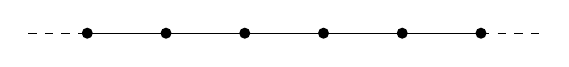
\begin{tikzpicture}
    \draw[dashed] (-.75, 0)--(0,0);
    \draw[dashed] (5,0)--(5.75, 0);
    \draw (0, 0)--(5, 0);
    \foreach \i in {0, 1, ..., 5} \fill (\i, 0) circle (2pt);
  \end{tikzpicture}

  \caption{\label{Z graf}Graf Cayleya grupy $\Z$ ma dwa końce.}
\end{figure}
który ma "dwa końce". Natomiast grupa wolna $F_2$ o dwóch generatorach ma "nieskończenie wiele końców" (rysunek \ref{graf F2}).
\begin{figure}[H]\center
  \begin{tikzpicture}
    \tikzmath {
      function drawLine (\x, \y, \scale, \step) {
        \step = \step -1;
        if \step >= 0 then {
          {
            \draw (\x, \y-0.8*\scale)--(\x, \y+0.8*\scale);
            \draw (\x-0.8*\scale, \y)--(\x+0.8*\scale, \y);
          };
          \scale = \scale *0.45;
          drawLine(\x - \scale, \y, \scale, \step);
          drawLine(\x + \scale, \y, \scale, \step);
          drawLine(\x, \y - \scale, \scale, \step);
          drawLine(\x, \y + \scale, \scale, \step);
        };
      };
      drawLine(0, 0, 4, 4);
    }
  \end{tikzpicture}
  \caption{\label{graf F2}Graf Cayleya grupy wolnej $F_2$ ma nieskończenie wiele końców.}
\end{figure}
Z drugiej strony, grupa $\Z^2$ ma jeden koniec: jeśli weźmiemy dwa bardzo odległe od siebie obszary, to one są ze sobą połączone, chociaż jest to połączenie "bardzo odległe" (obrazek \ref{graf Z2}).
\begin{figure}[H]\center
  \begin{tikzpicture}
    \tikzmath{
      for \x in {-3, ..., 3} {
        {
          \draw (\x, 3)--(\x, -3);
          \draw[dashed] (\x, 3)--(\x, 3.5);
          \draw[dashed] (\x, -3)--(\x, -3.5);
          \draw (-3, \x)--(3, \x);
          \draw[dashed] (-3.5, \x)--(-3, \x);
          \draw[dashed] (3, \x)--(3.5, \x);
        };
        for \y in {-3, ..., 3} {
          {\fill (\x, \y) circle (2pt);};
        };
      };
    }
    
    \draw[blue, thick, dashed] (-4, 0) to[out=-90, in=170]
      (-3.5, -4) to[out=-10, in=190] 
      (3.5, -4) to[out=10, in=-90]
      (4, 0);
    \draw[blue, thick, dashed] (-6, 0) to[out=-90, in=170]
      (-5.5, -5) to[out=-10, in=190]
      (5.5, -5) to[out=10, in=-90]
      (6, 0);

    \draw[orange, dashed, thick] (5, 0) ellipse (1 and 1.8);
    \draw[orange, dashed, thick] (-5, 0) ellipse (1 and 1.8);

    \node at (-6, 3) {\begin{varwidth}{3.3cm}\begin{center}\color{orange}dwa bardzo odległe obszary\end{center}\end{varwidth}};

    \draw[orange, ->, thick] (-7, 2.2) to[out=-90, in=180] (-6.2, 0);
    \draw[orange, ->, thick] (-4.3, 3.4) to[out=30, in=90] (5, 2);

    % \node[blue] at (0, -4.9) {połączone, choć nie bezpośrednio};
    \draw[decoration={text along path, text={połączone, choć nie bezpośrednio}, text align=center, text color=blue}, decorate] 
      (-3.5, -4.8) to[out=-10, in=190] (3.5, -4.8); 
  \end{tikzpicture}
  \caption{\label{graf Z2}Graf Cayleya grupy $\Z^2$ ma jeden koniec.}
\end{figure}
Każda przestrzeń skończona, np. graf Cayleya grupy skończonej, ma $0$ końców.

Chcemy z liczby końców przestrzeni (albo przestrzeni końców) uczynić tzw. niezmiennik asymptotyczny, czyli cechę niezmienną na quazi-izometrie właściwych geodezyjnych przestrzeni metrycznych, a co za tym idzie - przestrzeni skończenie generowanych.

\subsection{Granica odwrotna}

\begin{definition}{zbiór skierowany}{}
  Zbór z częściowym porządkiem $(\Lambda, \leq)$ jest \buff{skierowany}, gdy dla dowolnych $\lambda_1,\lambda_2\in\Lambda$ istnieje $\lambda\in\Lambda$ takie, że $\lambda\geq \lambda_1$ oraz $\lambda\geq \lambda_2$.
\end{definition}

% {\large\color{red}ciągi odwrotne}

\begin{definition}{system odwrotny}{}
  \buff{System odwrotny} nad zbiorem skierowanym $\Lambda$ to rodzina zbiorów 
  $$\mathfrak{X}:=\{X_\lambda\;:\;\lambda\in\Lambda \}$$
  oraz rodzina odwzorowań
  $$\mathcal{F}:=\{f_{\lambda\mu}:X_\mu\to X_\lambda\;:\;\lambda\leq\mu \}$$
  takich, że 
  \begin{enumerate}
    \item dla dowolnego $\lambda$ mamy funkcję identycznościową: $f_{\lambda\lambda}=id_{X_\lambda}$
    \item dla dowolnych $\lambda\leq\mu\leq\nu$ złożenia zachowują się dobrze: $f_{\lambda\nu}=f_{\lambda\mu}\circ f_{\mu\nu}$.
  \end{enumerate}
\end{definition}

Będziemy oznaczać: $\boldsymbol{\underline{X}:=(\Lambda, \mathfrak{X}, \mathcal{F})}$

\begin{definition}{granica odwrotna}{granica odwrotna}
  Granicą odwrotną systemu $\underline{X}$ nazywamy zbiór
  $$\varprojlim\underline{X}=\varprojlim(\Lambda, \mathfrak{X}, \mathcal{F}):=\{\xi\in\prod_{\lambda\in\Lambda}X_\lambda\;:\;(\forall\;\lambda'\leq\lambda)\;\xi_{\lambda'}=f_{\lambda'\lambda}(\xi_\lambda)\}.$$
  Elementy $\xi$ jak wyżej nazywamy \hl{niciami} (threads) w $\underline{X}$.
\end{definition}

% \begin{definition}{odwzorowania graniczne}{}
Odwzorowania 
$$f_\lambda:\varprojlim\underline{X}\to X_\lambda$$ 
takie, że $f_\lambda(\xi)=\xi_\lambda$ nazywamy \buff{odwzorowaniami granicznymi}.
O odwzorowaniach granicznych można myśleć jako o odwzorowaniach, które pytają "kim byłem w czasie $\lambda$".

\begin{center}
  \begin{tikzcd}
    X_1 & X_2 \arrow[l] & X_3\arrow[l] & X_4 \arrow[l] & ... \arrow[l]\\ 
        & & \varprojlim\underline{X}\arrow[ull]\arrow[ul]\arrow[u]\arrow[ur]\arrow[urr]
  \end{tikzcd}
\end{center}

Dla $\lambda\leq\mu$ diagram 
\begin{center}
  \begin{tikzcd}
    &\underset{\leftarrow}{\lim}\underline{X}\arrow[dl, "f_\lambda" above left]\arrow[dr, "f_\mu"]\\ 
    X_\lambda && X_\mu\arrow[ll, "f_{\lambda\mu}"]
  \end{tikzcd}
\end{center}
zawsze komutuje.

% \subsection{Toopologia granicy odwrotnej}

Kiedy zbiory $X_\lambda$ są przestrzeniami topologicznymi, zaś $f_{\lambda\mu}$ są ciągłe, to na granicy odwrotnej $\varprojlim\underline{X}$ rozważamy również topologię graniczną. Jest to topologia dziedziczona z topologii produktowej na $\prod_{\lambda\in\Lambda}X_\lambda$. 

\hl{Bazą tej topologii są zbiory postaci }\hl{$f_\lambda^{-1}(U)$ dla $\lambda\in\Lambda$ i otwartych $U\subseteq X$.}

\begin{fact}{}{}
  Granica odwrotna $\varprojlim\underline{X}$ jest:
  \begin{enumerate}
    \item domkniętym podzbiorem $\prod_{\lambda\in\Lambda}X_\lambda$, jeśli $X_\lambda$ są Hausdorffa,
      % gdy przestrzenie $X_\lambda$ są Hausdorffa, to $\varprojlim \underline{X}$ jest domkniętym podzbiorem w $\prod_{\lambda\in\Lambda}X_\lambda$.
    \item zwarta i metryczna, jeśli $X_\lambda$ takie są,
    \item zwarta i metryczna, jeśli $\Lambda$ jest przeliczalny, a $X_\lambda$ są skończone (z topologią dyskretną).
  \end{enumerate}
\end{fact}

W ostatnim przypadku $\varprojlim \underline{X}$ nie jest przestrzenią dyskretną, pomimo, że wszystkie zbiory po których bierzemy granicę takie były. Rozważmy następujący przykład, w którym $\Lambda=\N$, a wszystkie $X_\lambda$ są skończone dyskretne, natomiast $\varprojlim \underline{X}$ jest niedyskretne i nieskończone.

% Gdy przestrzenie $X_\lambda$ są zwarte i metryczne, to wówczas $\varprojlim\underline{X}$ też jest zwarta i metryczna. W szczególności, gdy $X_\lambda$ są skończone (z topologią dyskretną), zaś $\Lambda$ jest przeliczalny, to wówczas $\varprojlim\underline{X}$ jest \hl{przestrzenią zwartą i metryczną}. Na ogół nie jest też przestrzenią dyskretną, mimo że wszystkie zbiory po których bierzemy granicę takie były (bazą topologii są przeciwobrazy punktów $\{\xi\in\varprojlim\underline{X}\;:\;\xi_\lambda=x\}=f^{-1}_\lambda(x)$).

\begin{example}{}{}
  Niech $\Lambda=(\N, \leq)$ i niech $X_k$ będzie zbiorem wszystkich ciągów $0-1$ długości $k$. Dla $k\leq m$ rozważamy 
  $$f_{km}:X_m\to X_k$$
  będące obcięciem ciągu długości $m$ do początkowego ciągu długości $k$. Dostajemy wówczas system odwrotny $\underline{X}=(\N, \{X_k\}, \{f_{km}\})$ zbiorów skończonych. Wówczas $\varprojlim\underline{X}$ jest homeomorficzny ze zbiorem Cantora.
\end{example}

\subsection{Przestrzeń końców}

Na tym wykładzie będziemy zajmować się $X$, które są właściwymi geodezyjnymi przestrzeniami metrycznymi. Takimi przestrzeniami są np. grafy Cayleya grup skończenie generowalnych. Przez zbiór $\mathcal{K}$ będziemy rozumieć rodzinę wszystkich zwartych podzbiorów $K\subseteq X$ z porządkiem inkluzji.

% Będziemy zajmować się $X$ które są przestrzeniami metrycznymi, geodezyjnymi właściwymi, np. grafami Cayleya grup skończenie generowanych. $\mathcal{K}$ to będzie rodzina wszystkich zwartych podzbiorów $K\subseteq X$ z porządkiem inkluzji.

\begin{definition}{podzbiór współkońcowy}{}
  Podzbiór $M\subseteq\Lambda$ zbioru skierowanego $\Lambda$ nazywamy \buff{współkońcowym}, jeśli 
  $$(\forall\;\lambda\in\Lambda)(\exists\;\mu\in M)\;\lambda\leq\mu,$$ 
  wtedy $(M, \leq)$ też jest zbiorem skierowanym. Dla $\underline{X}=(\Lambda, \mathfrak{X}, \mathcal{F})$ niech 
  $$\underline{X}_{|M}=(M, \{X_\lambda\;:\;\lambda\in M\}, \{f_{\mu\mu'}\in\mathcal{F}\;:\;\mu,\mu'\in M\})$$
  będzie obcięciem $\underline{X}$ do $M$. Wtedy $\underline{X}_{|M}$ jest systemem odwrotnym nad $M$.
\end{definition}

\begin{fact}{}{}
  $$\varprojlim\underline{X}=\varprojlim\underline{X}_{|M}$$
  Przez bijekcją polegającą na obcinaniu nici do $M$. Jest ona jednocześnie homomorfizmem.
\end{fact}

\begin{conclusion}{}{} 
  Jeśli $X_\lambda$ są zwarte i metryczne, zaś $\Lambda$ posiada przeliczalny podzbiór współkońcowy, to $\varprojlim\underline{X}$ jest zwarta i metryczna.
\end{conclusion}

\begin{example}
Rodzina zbiorów zwartych $\mathcal{K}$ posiada współkońcowy podciąg $K_i:=B_{i\cdot R}(x_0)$ dla $R>0$ i pewnego $x_0\in X$.
  \end{example}
    
Dla dowolnego $K\in\mathcal{K}$ niech \hl{$\Pi_K^X$ będzie zbiorem nieograniczonych komponent spójności w dopełnieniu $X-K$}.

Przestrzeń geodezyjna jest lokalnie drogowo spójna i każda jej otwarta podprzestrzeń również jest lokalnie drogowo spójna. Stąd każde $X-K$ też jest lokalnie drogowo spójna. W lokalnie drogowo spójnych przestrzeniach komponenty spójności to to samo co komponenty drogowej spójności.\medskip

Dla $K\subseteq K'$, każda nieograniczona komponenta spójności $C'\subseteq X-K'$ zawiera się w dokładnie jednej nieograniczonej komponencie spójności $C\subseteq X-K$. Dostajemy więc odwzorowanie 
$$f_{KK'}:\Pi_{K'}^X\to \Pi_K^X$$
takie, że $f_{KK'}(C')=C$. 

Trójka $(\mathcal{K}, \{\Pi_K^X\;:\;K\in\mathcal{K}\},\{f_{KK'}\;:\;K'\subseteq K\})$ tworzy system odwrotny nad zbiorem skierowanym $\mathcal{K}$:
\begin{center}
  \begin{tikzcd}
    \Pi_K^X & \Pi_{K'}^X\arrow[l, "f_{KK'}"] & \Pi_{K''}^X\arrow[l, "f_{K'K''}"]
  \end{tikzcd}
\end{center}

\begin{fact}{}{}
  Dla każdego $K\in\mathcal{K}$ zbiór $\Pi_K^X$ jest skończony.
\end{fact}

\begin{proof}
  Weźmy dowolny $K\in\mathcal{K}$ i $x_0$ oraz $r$ takie, że 
  $$K\subseteq B_r(x_0).$$ 
  Niech $R>r$ i rozważmy zwartą kulę $B_R(x_0)$. Każda nieograniczona komponenta $C$ spójności w $X-K$ przecina niepusto sferę $S_R(x_0)$, bo $X$ jest geodezyjna, a więc lokalnie drogowo spójna...

  Zatem przekrój $C\cap B_R(x_0)$ jest niepusty. Wtedy rodzina 
  $$\{C\cap B_R(x_0)\;:\;C\text{ dowolna komponenta dopełnienia }X-K\}\cup \{\overline{B_R}(x_0)=B_R(x_0)-S_R(x_0)\}$$
  pokrywa $B_R(x_0)$. Dodatkowo, jest to otwarte pokrycie, bo komponenty spójności lokalnie spójnej przestrzeni są otwartymi podzbiorami w tej przestrzeni. 

  Ze zwartości $X$ to pokrycie posiada skończone podpokrycie, ale z drugiej strony każdy zbiór postaci $C\cap B_R(x_0)$ dla nieograniczonych komponent musi przetrwać w każdym podpokryciu, bo zawiera punkty które należą tylko do niego. Stąd nieograniczonych komponent jest skończenie wiele.
\end{proof}

\begin{definition}{przestrzeń końców}{}
  Zbiorem (przestrzenią) końców, $Ends(X)$, właściwej geodezyjnej przestrzeni metrycznej $X$ nazywamy granicę odwrotną
  $$\Ends(X)=\varprojlim(\Pi^X)=\varprojlim(\mathcal{X}, \{\Pi_K^X\}, \{f_{KK'}\}),$$
  gdzie $\Pi_K^X$ to nieograniczone komponenty w $X-K$.  Jest to zwarta przestrzeń metryczna.
\end{definition}

\begin{example}[m]
  \item $\Ends(\text{ograniczone}))=\emptyset$
  \item $\Ends(\Z^2)=\{\star\}$ to punkt w nieskończoności kraty
  \item $\Ends(\Z)=\{-\infty, \infty\}$ i jest równoliczny z $\Ends(\R)$
  \item zbiór końców drzewa $k$-regularnego, dla $k\geq 3$, jest izomorficzny ze zbiorem Cantora
  \item dla nieskończonych grup skończenie generowanych $G_1$, $G_2$ przestrzeń końców $\Ends(G_1\star G_2)$ jest nieskończonym zbiorem
\end{example}


